\section{Design Space Exploration on EBeSS}	\label{sec:exp}
%
Based on EBeSS, this section explores the performance of three energy behaviors of NVP and peripherals under unstable power supply profiles.

\begin{figure*}[!htpb]
	\centering
	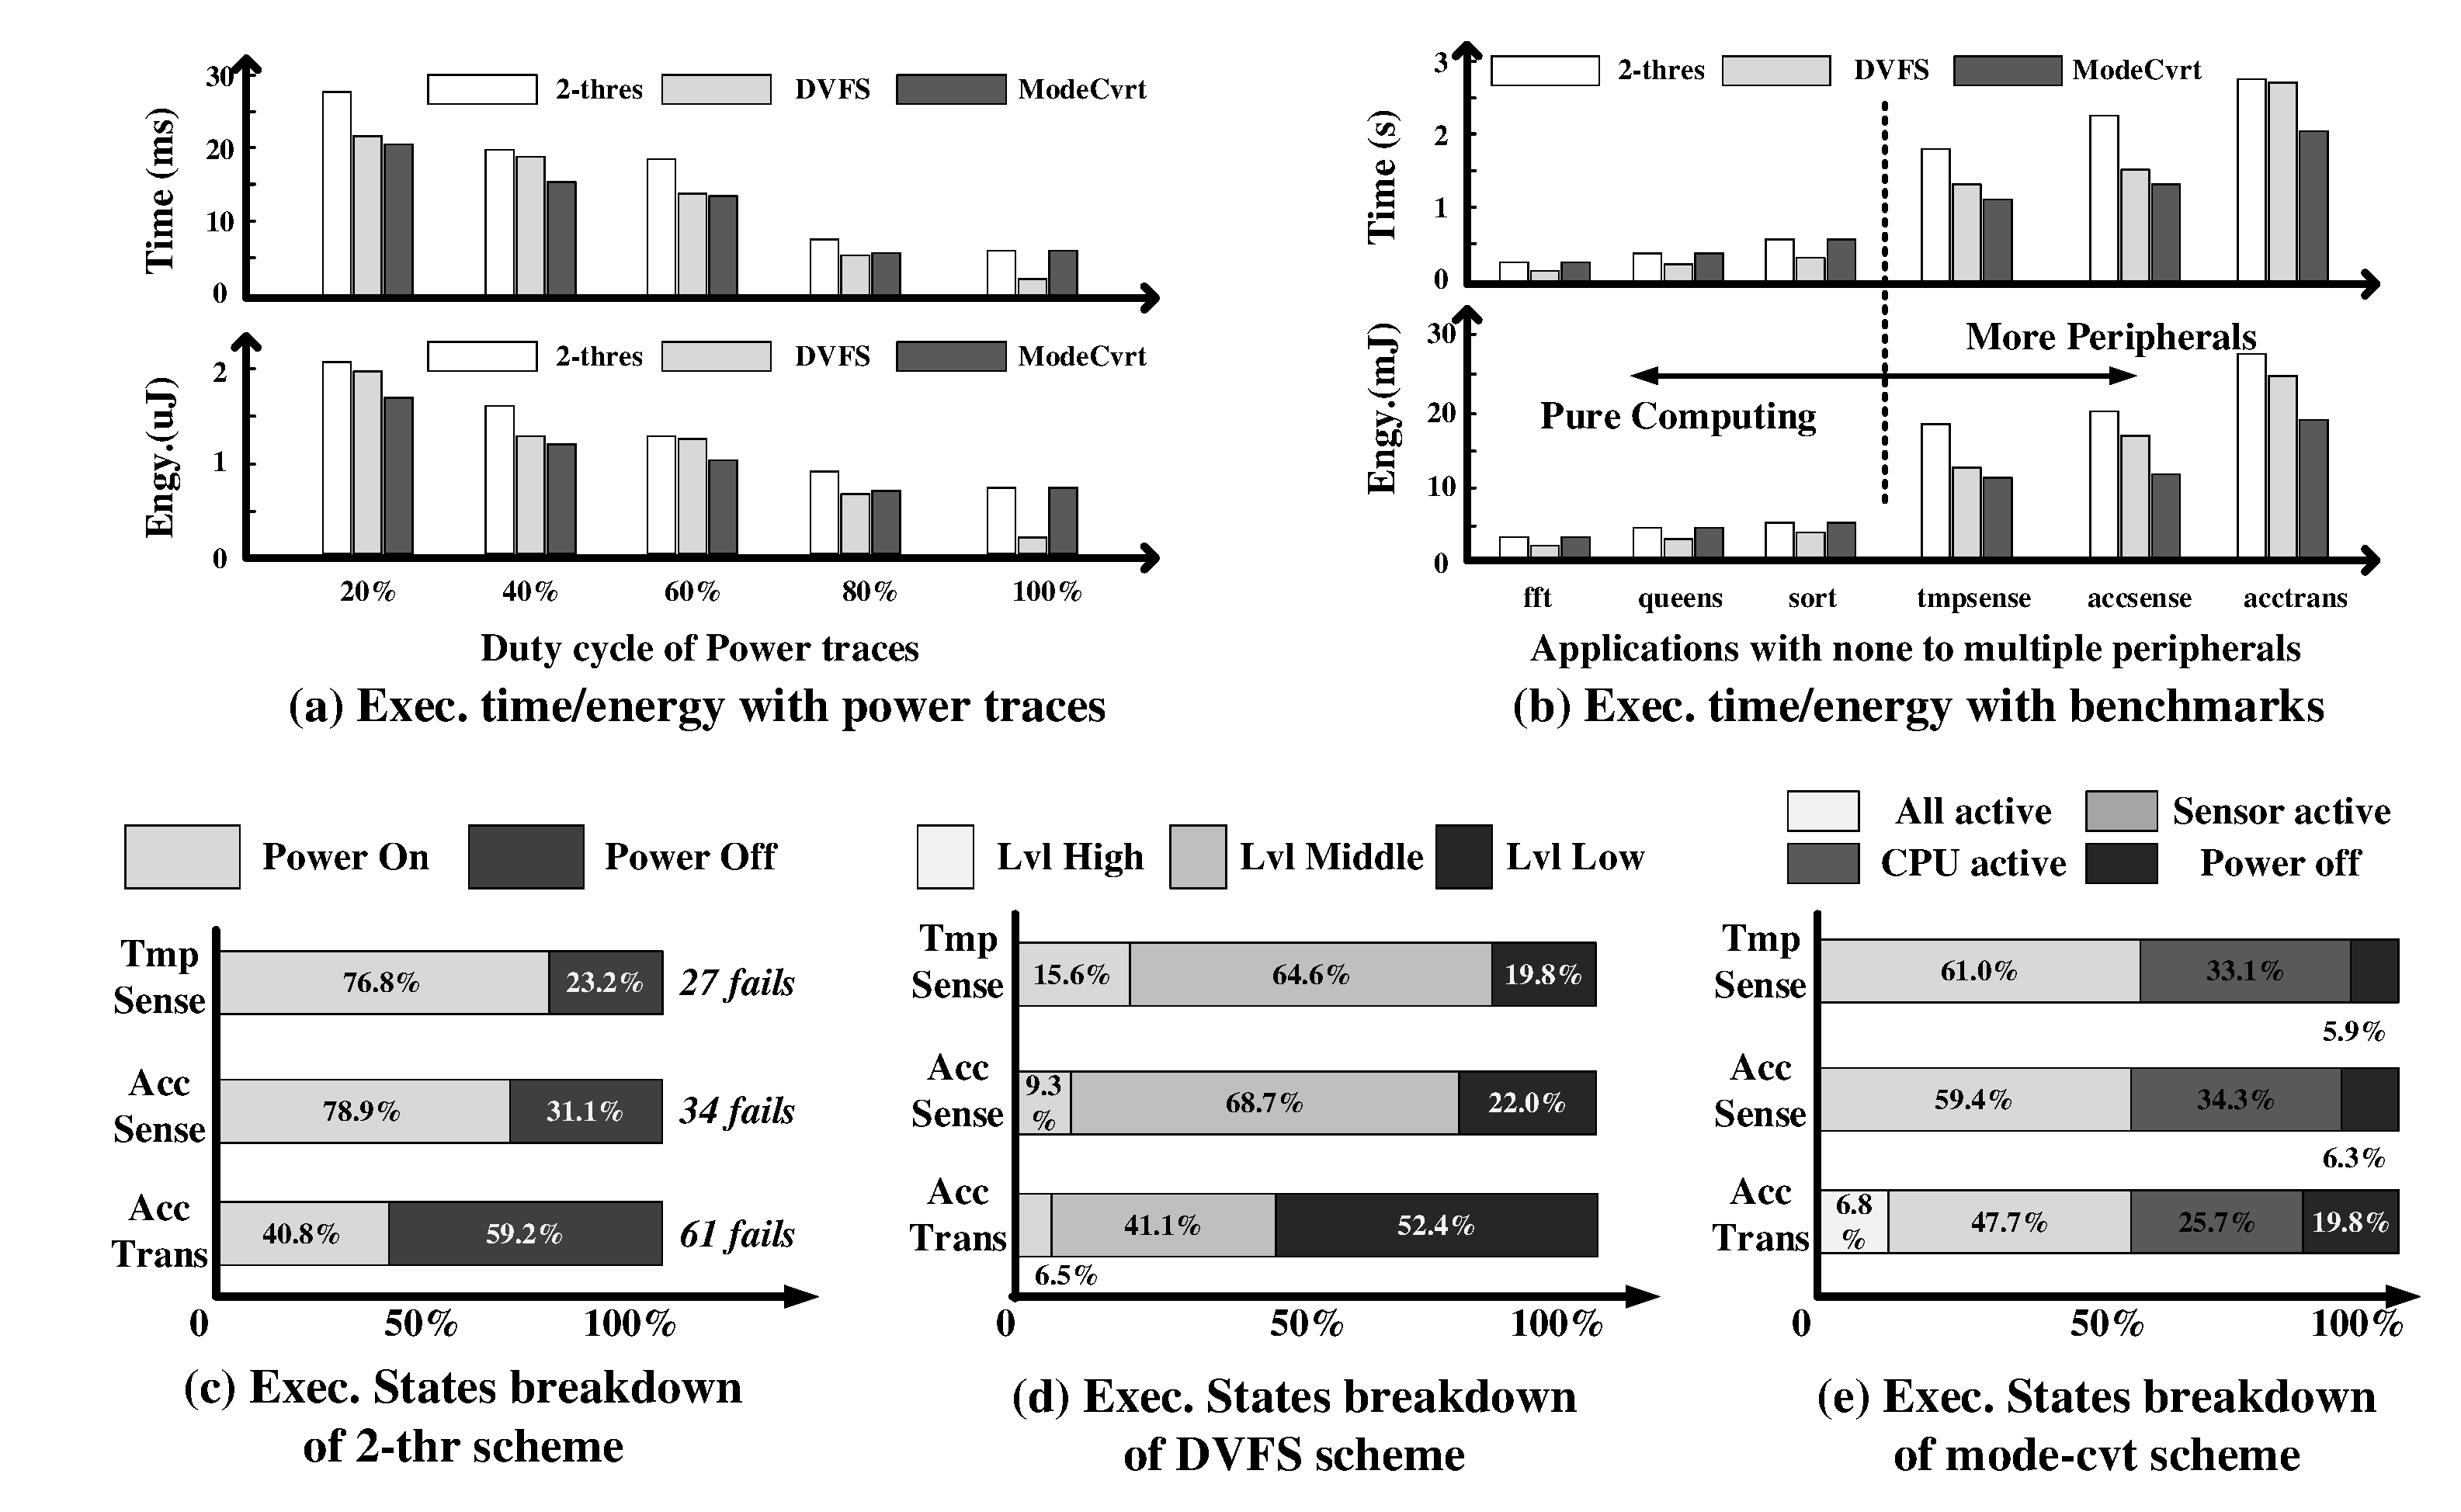
\includegraphics[width=1\textwidth]{ExperimentResults}
	\vspace{-15pt}
	\caption{Experiment Results. Figure (a) is the time and energy comparison of the energy behavior schemes executed under the power traces with different duty cycle. Figure (b) compares the execution results by executing 6 benchmarks which has different peripheral occupation. Figure (c)(d)(e) are execution states break downs of the three schemes executing three peripheral-contained benchmarks.}	\label{fig:ExperimentResults}
	\vspace{-5pt}
\end{figure*}


\subsection{Experiment Settings}	\label{sec:exp-settings}
%
The parameter settings are listed in Tab.~\ref{tab:exp-settings}.
EBeSS build an ARM based core simulator which executes at 1MHz.
This simulator contains a 16MB memory and a 2KB register file.
Three peripherals are connected in this system, that are a temperature sensor, an accelerometer and a radio transmitter.
The energy consumption values of these devices are listed in Tab.~\ref{tab:exp-settings}.
The power profiles are square waves with different duty-cycles.
The sample rate of each power profile is 10kHz.

Six benchmarks are used to explore the insight of energy behavior designs, as shown in Tab.~\ref{tab:exp-benchmarks}.
\emph{fft}, \emph{queens} and \emph{sort} are three computing dominated benchmarks which is executed on CPU with a few memory accessing operations.
\emph{TmpSense}, \emph{AccSense} and \emph{AccTrans} are three peripheral related benchmarks whose I/O operation occupation successively increases.

Three energy behavior schemes are analyzed in the explorations, that are \emph{2-thres}, \emph{DVFS}, and \emph{ModeCvrt}.
2-thres  is the example given in Sec.~\ref{sec:tech-example}, where two voltage thresholds are defined to manage system power on and off during execution.
As shown in Fig.~\ref{fig:EnergyBehaviorSchemes} (a), when the supply voltage grows above power-on threshold $V_{\text{on}}$, the system start to work.
When the supply voltage falls below power-off threshold $V_{\text{off}}$, the system is shutdown.
DVFS scheme provides three DVFS executing levels from high to low, where the levels with lower voltages are adopted in NVP when power supply voltage reduces. 
When the supply voltage changes across the thresholds ($V_{\text{d-1}}$, $V_{\text{d-2}}$, $V_{\text{d-3}}$), NVP changes the executing voltage and frequency as shown in Fig.~\ref{fig:EnergyBehaviorSchemes} (b).
ModeCvrt is a scheme that shuts down different hardware modules when the power supply is not enough.
There are three working modes and a power off mode.
When the supply voltage is higher than $V_{\text{m-3}}$, all the modules are active.
When the supply voltage is between $V_{\text{m-3}}$ and $V_{\text{m-2}}$, the RF transmitter is shutdown.
When the supply voltage is between $V_{\text{m-2}}$ and $V_{\text{m-1}}$, only the NVP is active and only computing operations are allowed.
When the supply voltage is below $V_{\text{m-1}}$, the system is powered off.

\begin{table}[t]
	\begin{center}
		\caption{Simulator Settings of the Explorations.} \label{tab:exp-settings}
		\vspace{-5pt}
		\Fsize{8}
		\renewcommand{\arraystretch}{1.5}
		%\setlength{\tabcolsep}{1pt}
		\begin{tabular}{IcIc|c|c|c|c|cI}
			\Xhline{1.2pt}
			\multirow{2}[0]{0.15cm}{\rotatebox{90}{CPU\ }}
					& ISA		& Freq.	& power	& Mem	& RegFile	& Cap. \\
			\cline{2-7}
					& ARM	& 1MHz	& 0.16mW	& 16MB	& 2KB		& 10$\mu$F \\


			\Xhline{1.2pt}
			\multirow{3}[0]{0.15cm}{\rotatebox{90}{Peripheral\ }}
					& \multicolumn{2}{c|}{Tmp. Sensor}	& \multicolumn{2}{c|}{Acc. Sensor}	& \multicolumn{2}{cI}{RF Trans.} \\
			\cline{2-7}
					& Active	& Idle				& Active	& Idle			& Active	& Idle \\
			\cline{2-7}
					& 6.55mW	& 0.33mW			& 2.86mW	& 0.50mW		& 39.6mW	& 0.65mW \\
			\Xhline{1.2pt}
		\end{tabular}
	\end{center}
	\vspace{-10pt}
\end{table} 
\begin{table}[t]
	\begin{center}
		\caption{Benchmarks Used in Energy Behavior Exploration.} \label{tab:exp-benchmarks}
		\vspace{-5pt}
		\Fsize{8}
		\renewcommand{\arraystretch}{1.5}
		%\setlength{\tabcolsep}{1pt}
		\begin{tabular}{IcIcIc|c|c|cI}
			\Xhline{1.2pt}
			\multirow{2}[1.2]{*}{App.}	& \multirow{2}[1.2]{*}{Type}	& \multicolumn{4}{cI}{Hardware Module Used} \\
			\cline{3-6}
							&					& CPU\&Mem.	& Tmp. Sen.	&Acc.	Sen.	& Trans. \\

			\Xhline{1.2pt}
			fft				& comp.				& $\surd$		& $\times$	& $\times$	& $\times$ \\

			\Xhline{1.2pt}
			queens				& comp.				& $\surd$		& $\times$	& $\times$	& $\times$ \\

			\Xhline{1.2pt}
			sort				& comp.				& $\surd$		& $\times$	& $\times$	& $\times$ \\

			\Xhline{1.2pt}
			TmpSense			& comp.				& $\surd$		& $\surd$	& $\times$	& $\times$ \\

			\Xhline{1.2pt}
			AccSense			& comp.				& $\surd$		& $\surd$	& $\surd$	& $\surd$ \\

			\Xhline{1.2pt}
			AccTrans			& comp.				& $\surd$		& $\surd$	& $\surd$	& $\surd$ \\

			\Xhline{1.2pt}
		\end{tabular}
	\end{center}
	\vspace{-10pt}
\end{table} 

\begin{figure}[htpb]
	\centering
	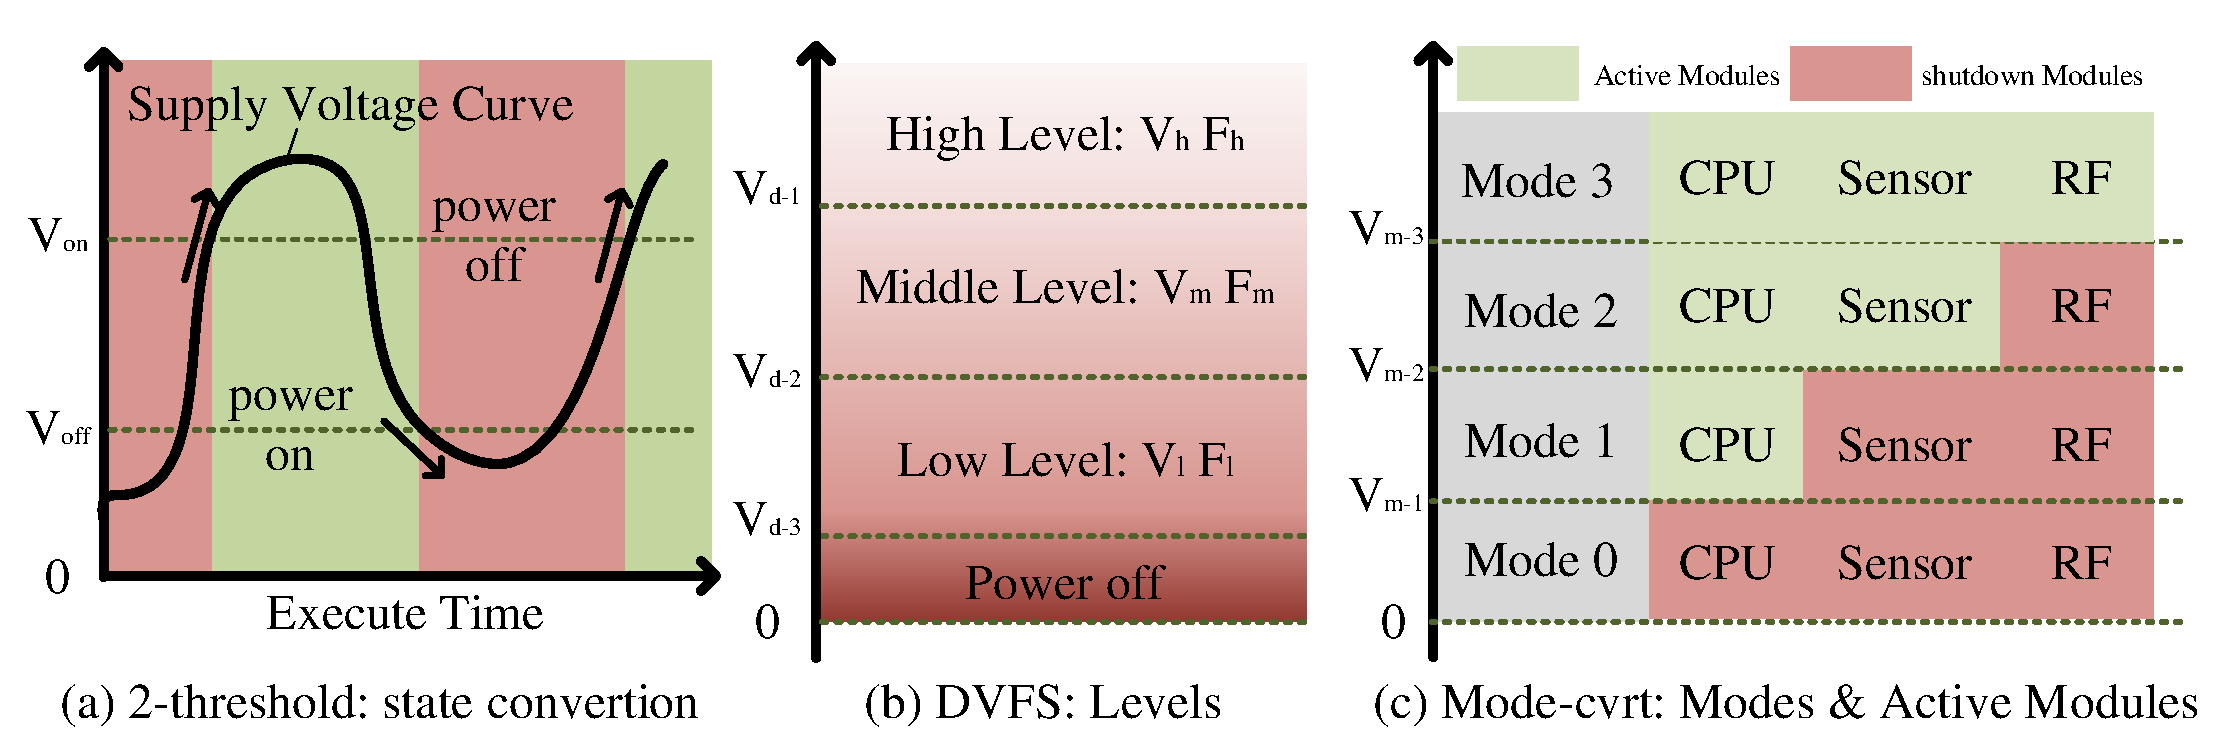
\includegraphics[width=0.5\textwidth]{EnergyBehaviorSchemes}
	\vspace{-20pt}
	\caption{The work flow of virtual devices w and w/o power failures.}	\label{fig:EnergyBehaviorSchemes}
	\vspace{-5pt}
\end{figure}

Based on this simulator and the configurations, we analyzes the performance of these energy behavior designs with different power profiles and applications. 


\begin{comment}
To illustrate the difference among these energy behavior schemes, \emph{TmpSense} is executed peridically in 2 minutes under a real power trace to compare the execution procedure and time.
%Fig.~\ref{fig:ExperimentResults} (a) shows task progress comparison using these three energy behavior designs.
Using the 2-thres scheme, the system frequently falls into power failures during execution. 
287 groups of temperature data are collected in 2 minutes.
DVFS level reduces the probability of power failures during the execution but induces lower execution speed when supply voltage is low.
Compared with 2-thres scheme, DVFS enhanced the executing efficiency by 30\%, which collects 373 groups of temperature data.
The ModeCvrt scheme is designed base on the idea of power gating, which reduces the leakage power when a hardware module is not used.
In this way, more energy is saved and the data collection efficiency is improve by 21.2\% (347 groups).
\end{comment}







\subsection{Impact of Power Profiles on Energy Behavior Design}	\label{sec:exp-power}
%
Power supply is one of the most critical impact that affect the execution efficiency of the energy behavior schemes.
By scanning the duty cycle of the square wave, power traces with different energy intensity is generate to power the system.
Fig.~\ref{fig:ExperimentResults} (a) shows the energy consumption and the execution time to complete the TmpSense benchmark.
With more efficient power supply, DVFS achieve higher executing speed than the other two schemes.
An interesting observation is that, although more energy is cost to complete the same task with high DVFS level, DVFS scheme can still achieve higher energy efficiency.
The reason is that, other schemes waste more energy when the capacitor is fully charged, while DVFS has the ability to take advantage of the sufficient supply power which finally increases the energy efficiency.

When the energy supply is insufficient, DVFS and ModeCvrt has similar performance to deal with the low power supply.
With the low DVFS level, the system keeps progress with low CPU power consumption and low execution speed.
On the other side, ModeCvrt has the ability to use peripheral more energy efficiently by reducing the power leakages when these devices are not executing.
Generally, compared with 2-thres, DVFS and ModeCvrt has 22.1\% and 17.7\% of performance improvement in averages, and can reduce the power consumption by 24.2\% and 21.9\% in average.






\subsection{Impact of Applications on Energy Behavior Design}	\label{sec:exp-app}
%
Application is another important factor that affect the executing performance and energy efficiency of the energy behaviors.
Applications in the energy harvesting system contains the computing operations executed on NVP and the I/O operations executed on the peripherals.
Since the energy behavior schemes have different adjustment priorities, applications with different I/O operation occupations will have different performance improvements adopting these energy behavior designs.

In this part, benchmark with different I/O operation occupations are used.
Fig.~\ref{fig:ExperimentResults} (b) shows the time and energy comparison of the energy behavior schemes with these benchmarks.
Results show that, with more peripherals used, ModeCvrt has significant energy saving and executing speed improvements.
In this condition, DVFS has little improvements because the power consumption of NVP is not dominating when more peripherals are used.
DVFS is superior in executing the pure computing benchmarks because its objective is to adjust the execution states of the processor.
However, with no peripheral, ModeCvrt lose its advantages to execute the computing tasks and has similar performance with 2-thres.

Fig.~\ref{fig:ExperimentResults} (c-f) show the execution state breakdowns of the three energy behavior schemes executing three benchmarks.
2-thres scheme leads to lots of power failures more than other two modules.
Because of large energy consumption, AccTrans spends most of the time in power off mode to charge the energy storages.
DVFS is also affected by peripherals.
Although DVFS focus on the execution of CPU, more peripherals affect the total energy consumption and leads to more low voltage execution time.
ModeCvrt performs better because the power gating strategy is more suitable for the peripherals by reducing the peripheral leakages.

\subsection{Exploration Conclusion}	\label{sec:exp-sum}
%
In conclusion, experiment explores the affect of the power supply density and the application types. 
Results show that, DVFS has the ability to take better usage of the too low and the too high energy supply.
On the other side, ModeCvrt and DVFS have the advantages in adjusting the energy usage of CPU and peripherals, respectively.
When the computing operations is dominating, DVFS has better performance to take fully usage of power supply.
When the I/O operations are dominating, ModeCvrt is the better choice to avoid the leakages of the idle peripherals.